\chapter{Introdução ao Jamovi}

\section{O que é o Jamovi?}

O jamovi é um software estatístico com interface gráfica. É um software relativamente novo, se comparado com os seus concorrentes como o SPSS, SAS e PSPP. Com o jamovi você consegue ter um ambiente de fácil aprendizado e fácil manuseio, pois é possível integrar a facilidade do ambiente gráfico, com o poder da linguagem R para a automação de trabalhos.

Além das análises estatísticas convencionais, tais como: estatística descritiva, tabelas cruzadas, boxplot, etc. É possível desenvolver modelos matemáticos. Assim, podemos definir o jamovi como uma solução completa para análises quantitativas e qualitativas com o uso da matemática e estatística. Um software estatístico completo e gratuito.

\begin{figure}[H]
    \centering
    \caption{Captura de Tela do Jamovi}
    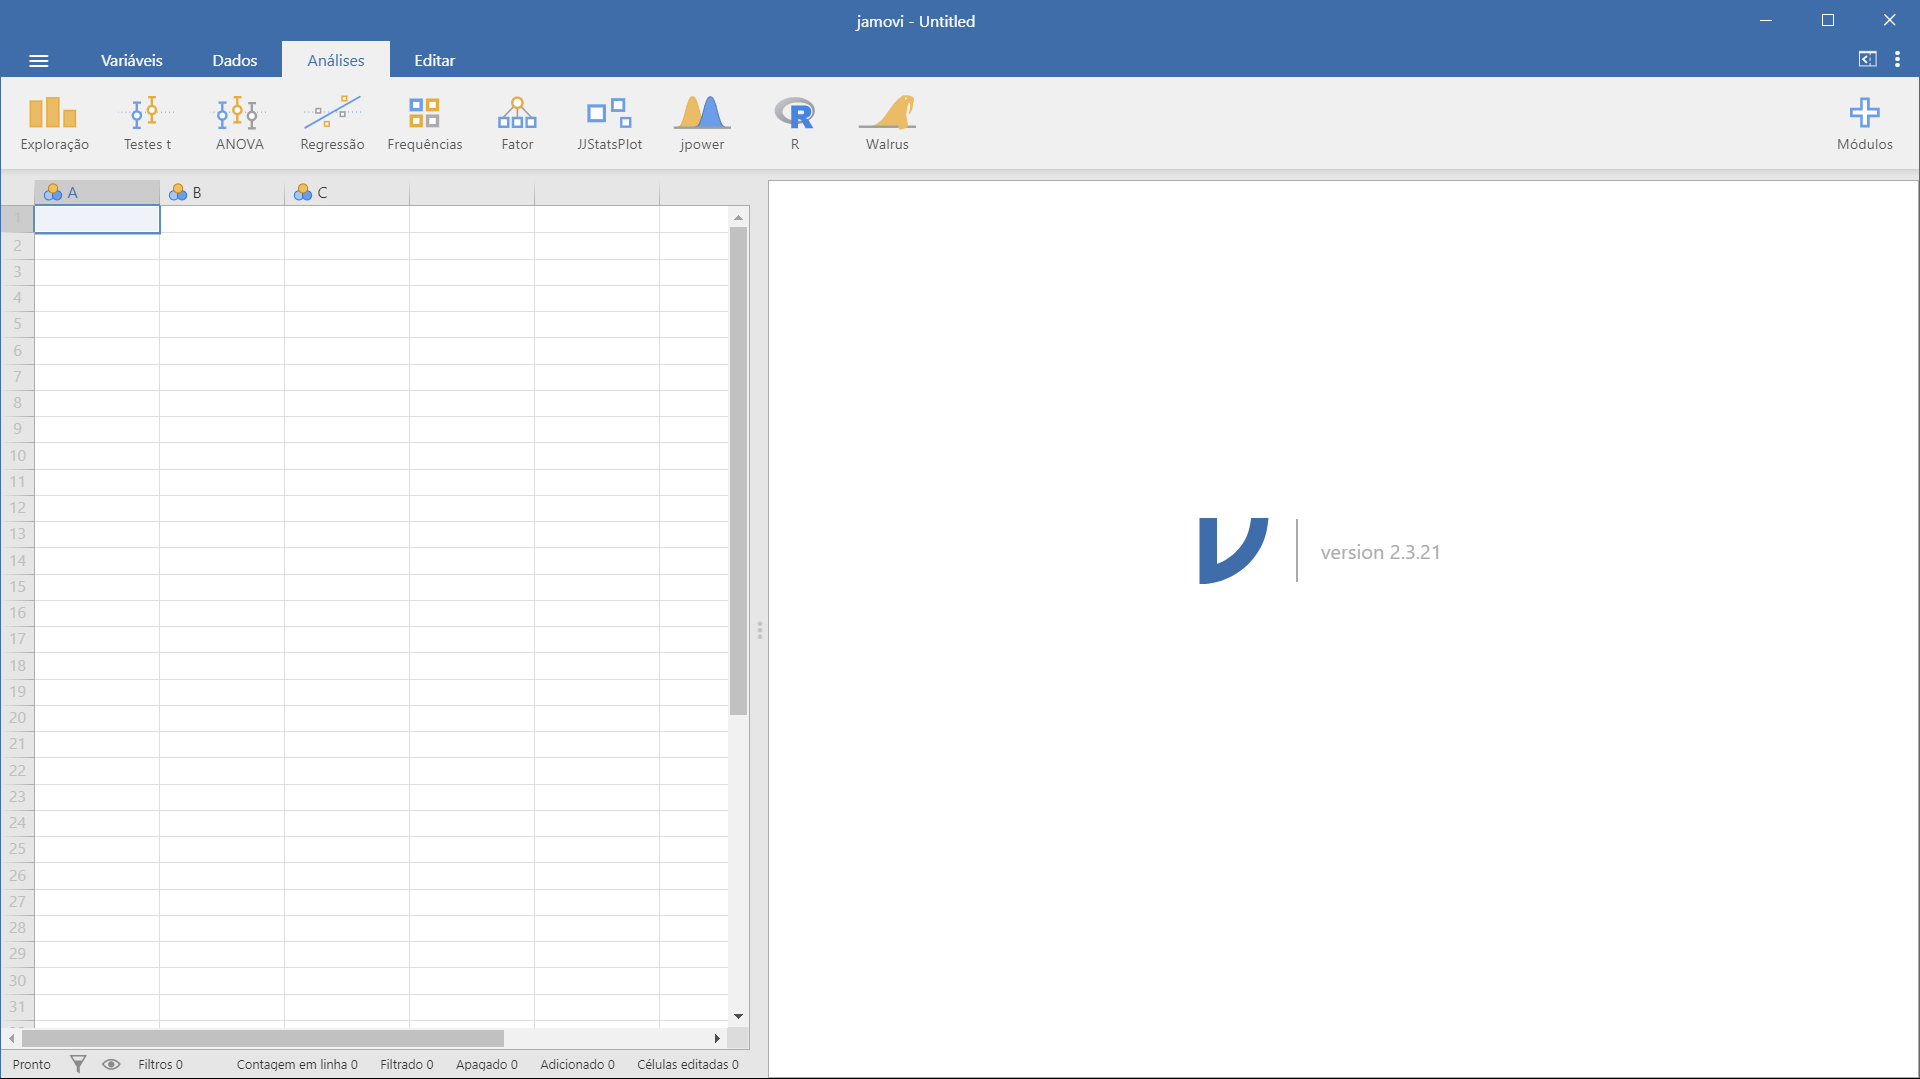
\includegraphics[width=\textwidth]{imagens/cap_1/captura_tela_jamovi.png}
    \label{fig:captura_tela_jamovi}
  \end{figure}

\subsection{Um software estatístico completo}

O jamovi é um dos softwares mais completos da atualidade. Sua interface gráfica e a integração com a linguagem de programação R, faz com que o programa seja capaz de realizar todas as análises, das mais simples até as mais importantes

Além de ser completo é um software open source e gratuito. Isso significa que você não precisa se preocupar em comprar licença e/ou fazer assinaturas. Além de ser gratuito, o fato de os códigos serem abertos, permite que todos e todas possam verificar diretamente no código fonte como o programa foi escrito, trazendo mais transparência e segurança para os(as) usuários(as)

\subsection{Estatística com interface gráfica}

Uma das principais barreiras para várias pessoas que desejam estudar estatística é a programação. Geralmente os(as) alunos(as) que estão começando a estudar estatística, estão começando também a ter o primeiro contato com a linguagem de programação

Uma das principais vantagens do Jamovi é sua interface gráfica. Com ela, o(a) aluno(a) que está começando nos estudos de estatística, pode se concentrar apenas no estudo teórico, deixando para outro momento o estudo da programação. Dessa forma, o jamovi é uma das melhores alternativas de software para estudos em estatística, pois permite que o(a) aluno(a) possa ver os resultados em tempo real, sem a necessidade de aprender os comandos de uma linguagem

\subsection{Software Modular}

O jamovi é um software modular. Isso significa que você pode instalar complementos, ou módulos de acordo com a sua necessidade. Diferentemente do SPSS, por exemplo, com o Jamovi você tem a liberdade de instalar somente os módulos que você precisa; algo que não é possível fazer no SPSS.

A liberdade de poder instalar os módulos, faz do Jamovi um software leve e personalizável. Além disso, a comunidade está ativamente desenvolvendo novos módulos, o que faz com que o Jamovi seja cada vez mais completo e flexível para atender diversos usuários

